\documentclass[journal]{IEEEtran}

%%%%%%%%%%%%%%%%%%%%%%%%%%%%%%%%%%%%%%%%%%%%%%%%%%%%%%%%%%%%%%%%%%%%%%%%%%%%%%%%
%
% Package
%
%%%%%%%%%%%%%%%%%%%%%%%%%%%%%%%%%%%%%%%%%%%%%%%%%%%%%%%%%%%%%%%%%%%%%%%%%%%%%%%%
\usepackage{ifpdf}
\ifCLASSINFOpdf
  \usepackage[pdftex]{graphicx}
  % declare the path(s) where your graphic files are
  % \graphicspath{{../pdf/}{../jpeg/}}
  % and their extensions so you won't have to specify these with
  % every instance of \includegraphics
  \DeclareGraphicsExtensions{.pdf,.jpeg,.png}
\else
  % or other class option (dvipsone, dvipdf, if not using dvips). graphicx
  % will default to the driver specified in the system graphics.cfg if no
  % driver is specified.
  \usepackage[dvips]{graphicx}
  % declare the path(s) where your graphic files are
  % \graphicspath{{../eps/}}
  % and their extensions so you won't have to specify these with
  % every instance of \includegraphics
  \DeclareGraphicsExtensions{.eps}
\fi

\usepackage[utf8]{inputenc}
\usepackage[T1]{fontenc}
\usepackage[french, english]{babel}
\usepackage{cite}
\usepackage{caption}
\usepackage{amsmath,amsfonts,amssymb}
\usepackage{subcaption}
\usepackage{array}
\usepackage{color}
\usepackage{float}
\usepackage{multicol}
\usepackage[]{algorithm2e}
\usepackage{hyperref}
\usepackage{fancyhdr}
%
% correct bad hyphenation here
\hyphenation{op-tical net-works semi-conduc-tor}

\DeclareMathOperator*{\argmin}{arg\,min}
\DeclareMathOperator*{\argmax}{arg\,max}

\begin{document}
%\pagestyle{plain}
%\pagenumbering{arabic}

%%%%%%%%%%%%%%%%%%%%%%%%%%%%%%%%%%%%%%%%%%%%%%%%%%%%%%%%%%%%%%%%%%%%%%%%%%%%%%%%
%
% Title
%
%%%%%%%%%%%%%%%%%%%%%%%%%%%%%%%%%%%%%%%%%%%%%%%%%%%%%%%%%%%%%%%%%%%%%%%%%%%%%%%%
\title{Stability and Performance of Coalitions of Prosumers Through Diversification in the Smart Grid}

%%%%%%%%%%%%%%%%%%%%%%%%%%%%%%%%%%%%%%%%%%%%%%%%%%%%%%%%%%%%%%%%%%%%%%%%%%%%%%%%
%
% Authors
%
%%%%%%%%%%%%%%%%%%%%%%%%%%%%%%%%%%%%%%%%%%%%%%%%%%%%%%%%%%%%%%%%%%%%%%%%%%%%%%%%
\author{Nicolas Gensollen, Vincent Gauthier, Monique Becker and Michel Marot
%\IEEEauthorblockA{CNRS UMR 5157 SAMOVAR, \\
%Telecom SudParis/Institut Mines Telecom\\
%Email: \{nicolas.gensollen, vincent.gauthier, michel.marot, monique.becker\}@telecom-sudparis.eu}}
\thanks{Authors are with CNRS UMR 5157 SAMOVAR, Telecom SudParis/Institut Mines Telecom, e-mail: (\{nicolas.gensollen, vincent.gauthier, michel.marot, monique.becker\}@telecom-sudparis.eu)}}%


\maketitle

%%%%%%%%%%%%%%%%%%%%%%%%%%%%%%%%%%%%%%%%%%%%%%%%%%%%%%%%%%%%%%%%%%%%%%%%%%%%%%%%
%
% Abstract
%
%%%%%%%%%%%%%%%%%%%%%%%%%%%%%%%%%%%%%%%%%%%%%%%%%%%%%%%%%%%%%%%%%%%%%%%%%%%%%%%%
\begin{abstract}
In the context of the smart grid, we propose in this paper an algorithm that forms coalitions of agents, called prosumers, that both produce and consume. It is designed to be used by aggregators that aim at selling aggregated surplus of production of the prosumers they control. We rely on real weather data sampled across stations of a given territory in order to simulate realistic production and consumption patterns for each prosumer. This enables us to capture geographical correlations among the agents while preserving the diversity due to different behaviors. As aggregators are bound to the market operator by a contract, they seek to maximize their offer while minimizing their risk. The proposed graph based algorithm takes the underlying correlation structure of the agents into account and outputs coalitions with both high productivity and low variability. We show that the resulting diversified coalitions are able to generate higher benefits on a constrained energy market, and are more resilient to random failures of the agents.
\end{abstract}

\IEEEpeerreviewmaketitle

{\bf Keywords:} prosumers, coalition formation, correlation, stability, clique expansion, electricity market
%%%%%%%%%%%%%%%%%%%%%%%%%%%%%%%%%%%%%%%%%%%%%%%%%%%%%%%%%%%%%%%%%%%%%%%%%%%%%%%%
%
% Section I: Introduction
%
%%%%%%%%%%%%%%%%%%%%%%%%%%%%%%%%%%%%%%%%%%%%%%%%%%%%%%%%%%%%%%%%%%%%%%%%%%%%%%%%
\section{Introduction}
\label{sec:introduction}

%The recent developments in the smart grid area, such as demand side management mechanisms, storage efficiency, or communication architectures to name a few, sketch a new power system. 

%Bidirectional power flows, storage, and distributed production are characteristics of smart grid systems. Nodes that were simply pure loads yesterday could behave tomorrow as generators or loads depending on weather conditions.

%Bidirectional power flows, storage, and efficient use of information are some of the key principles that will enable this transition. Since production could be located down to the very end of the distribution networks, nodes that were simply pure loads yesterday could behave tomorrow as generators or loads, further complicating energy usages. 

Achieving a successful energetic transition through a smarter and greener electricity grid is a major goal for the 21st century. It is assumed that such smart grids will be characterized by bidirectional electricity flows coupled with the use of small renewable generators and a proper efficient information system. All these bricks might enable end users to take part in the grid stability by injecting power, or by shaping their consumption against financial compensation.

In this paper, we consider agents in the distribution network that own both renewable distributed energy resources (DER) and loads. We will refer to these agents as prosumers \cite{Rathnayaka2012} in the future. If a prosumer produces more than he consumes, he might be willing to sell power. We thus assume the existence of an energy market where producers post a production capacity for an upcoming period, and buyers decide what bids to purchase. When the production is stochastic, as it can be with DER, this approach gets more complicated and risk should be quantified and taken into account. We thus assume the existence of a market operator who constrains the market entrance. As single agents might not be productive or reliable enough, aggregators managing large portfolios of prosumers are more likely to enter such markets. While there exists several models for fixing prices and organizing bids in such stochastic settings, the present work does not focus on transactions on the market. Instead, we study how aggregators can manage their portfolios as to maximize the production that they offer, given that such production is stochastic by nature. A key point of this work is then to merge the interests of the market operator and aggregators in a single utility function. While the aggregators intend to maximize their benefits with better contracts, the operator concerns are related to the quality and reliability of the market supply (more information about the scenario can be found in \cite{Europe} page 67-68). If a buyer purchases a contract, the corresponding aggregator has to inject the contracted amount of power at any time of the contract, exposing himself to financial penalties if he deviates. Since prosumers use renewables, we are concerned with the probability that the production falls below the contract value. In this case, storage or demand side managment might be solutions to avoid penalties, but this probability should still be maintained low. 

We use a coalitional framework in order to model aggregators. It is known that diversification of the assets is a way of minimizing risks when building a portfolio. We thus expect more stable and predictable energy productions for aggreagtors than for single agents. Nevertheless, all coalitions are not equally stable or productive. Attention should thus be paid to the aggregation step. Recall that prosumers have both consumption and production components, each depending on location and time, meaning that there are complex underlying correlations between the agents. This is a central topic of this paper : given N prosumers, what coalitions should be formed so that the compromise between expected production and variability is optimized ?

We will see that the variability in the production of the aggregators can be quantified to a certain extent by the correlation among the agents within the coalitions. Understanding the correlation relationships among the agents can thus give an indication about what coalitions to form and how much they should sell on the market. More precisely, we use a graph representation of the correlation structure to gain insight about the expected production to risk ratios of different coalitions. We build a framework in which the market operator specifies both the minimum production acceptable to enter the market and restrain the amount of risk he is willing to accept. We then propose a graph heuristic that uses decorrelated cliques in order to form diversified productive and stable coalitions, and we compare the results with other formation strategies (see section \ref{sec:results}). Rather than maximizing the profit of each agent in the grid (prosumers and operator), our algorithm tries to form the most productive coalitions given a maximum amount of acceptable risk. In other words, it tries to maximize aggregators' profits without considering individual retributions to single agents. Furthermore, the pricing strategies for both the prosumer and the grid is beyond the scope of this paper.  

Because agents are susceptible to fail for diverse reasons, the propensity of the system to undertake these failures is critical \cite{Pahwa}. We therefore investigate in this paper the resilience of the coalitions when prosumers fail. Despite the fact that losing agents is usually detrimental to the coalitions, we will see that the coalitions formed with our algorithm tend to be less impacted by random failures.

The paper is organized as follows, section \ref{sec:related} gives a brief overview of the related literature, section \ref{sec:data} clarifies how we generated realistic prosumer production traces based on weather data. In section \ref{sec:notations}, we define most of the notations and explain why correlation between prosumers is a quantity of interest for our objective. Based on the conclusions of section \ref{sec:notations}, we develop in section \ref{sec:utility} a utility function quantifying how much power a coalition can announce on the market given an accepted risk level. We then develop, in section \ref{sec:forming} a greedy optimization algorithm that uses decorrelated cliques as inputs and improves their utility over a correlation-constrained environment. Finally, section \ref{sec:results} provides some results both on performance of the method and resilience of the coalitions formed. The overall process is illustrated on figure \ref{fig:process}.


%%%%%%%%%%%%%%%%%%%%%%%%%%%%%%%%%%%%%%%%%%%%%%%%%%%%%%%%%%%%%%%%%%%%%%%%%%%%%%%%
%
% Section II: Related Work
%
%%%%%%%%%%%%%%%%%%%%%%%%%%%%%%%%%%%%%%%%%%%%%%%%%%%%%%%%%%%%%%%%%%%%%%%%%%%%%%%%

\section{Related Work}
\label{sec:related}


Assuming a large penetration of DER, it is expected that the managment of the system would have to evolve as to copy with the large amount of unpredictable small generators. In \cite{Zhang2013}, the authors introduce a distributed energy management system with a high use of renewables such that power is scheduled in a distributed fashion. Allowing the formation of coalitions whose participants commit to achieving some objective against a reward appears also as a promising approach. Nevertheless, for these structures to be stable toward defection, agents should have an incentive to join, and cooperate. Coalition formation is therefore usually studied through the framework of game theory \cite{Saad2011}. In this direction, \cite{Nguyen2013} introduces an agent-based strategy for managing DER aiming at optimal performance in the electricity supply system.

Since most of the DER have a stochastic production, maintaining the system equilibrium in these conditions is a complicated task. It is often assumed that electricity storage will provide some possibilities in order to copy with the uncertainties. In \cite{Shadmand2014} the optimal storage capacity problem is addressed. There is indeed an interesting trade-off between the costs of the equipments and the expected availability of power. The authors develop a framework that enables them to exhibit a Pareto front of efficient solutions.

In addition to storage and distibuted algorithms, prediction techniques of the upcoming load curves and weather conditions are of paramount importance. Combining all these technologies could enable aggregators to quantify their expected production and the inherent risk that comes with it. The optimization of expected returns to risk is a traditional goal in finance, and a wide literature exists on this topic. It is well-known for instance, that the more risk one is willing to accept, the higher his potential gains. On the contrary, when investing exclusively on low risks assets, one should expect relatively small gains. This trade-off is formalized in the Markowitz' portfolio theory \cite{Markowitz1959}. More precisely, given a set of assets for which we have some historic data of returns, the objective is to find a linear combination of these assets (the so-called portfolio) which maximizes the expected value while minimizing the variance of the portfolio's return. Markowitz's answer is a set of efficient portfolios that all optimize in some sense this trade-off. If one is able to put a number on his risk acceptance or on the target expected return, the corresponding efficient portfolio is a priori the best option. One of the most controversial assumptions in the portfolio theory is that returns are jointly normally distributed (or, at least, that the returns distribution is jointly elliptical). Some economist have pointed out the fact that this assumption might not capture well the reality of financial markets \cite{doi:10.1142/S0219024912500197}. Nevertheless, one of the key point in the Markowitz theory is to consider explicitly the correlation between the assets since they impact directly the variances of the portfolios. Since the work of \cite{Mantegna1999}, an interesting approach consists in computing a distance metric based on the correlation coefficients in order to organize the series in a correlation graph. Nodes represent the series considered while the edges are weighted by the metric. Because the metric can be computed for all pairs, these graphs are complete and of little use as is. Historically, the approach used by \cite{Mantegna1999} was to compute a minimum spanning tree as to obtain a hierarchical clustering of the series. Later on, it was pointed out that, by definition, a spanning tree could not capture the underlying clustering structure hidden in the correlation graph. In this paper, we use another classical filtering technique called $ \epsilon $-graph \cite{Garas2008}. It consists in selecting a threshold $ \epsilon $, and filtering out edges with smaller weights. As we will see further in this paper, this approach has the advantage of preserving clusters of correlated series.


%%%%%%%%%%%%%%%%%%%%%%%%%%%%%%%%%%%%%%%%%%%%%%%%%%%%%%%%%%%%%%%%%%%%%%%%%%%%%%%%
%
% Section III: Generating realistic prosumer patterns
%
%%%%%%%%%%%%%%%%%%%%%%%%%%%%%%%%%%%%%%%%%%%%%%%%%%%%%%%%%%%%%%%%%%%%%%%%%%%%%%%%

\section{Generating realistic prosumer patterns}
\label{sec:data}


\begin{figure}
	\begin{center}
		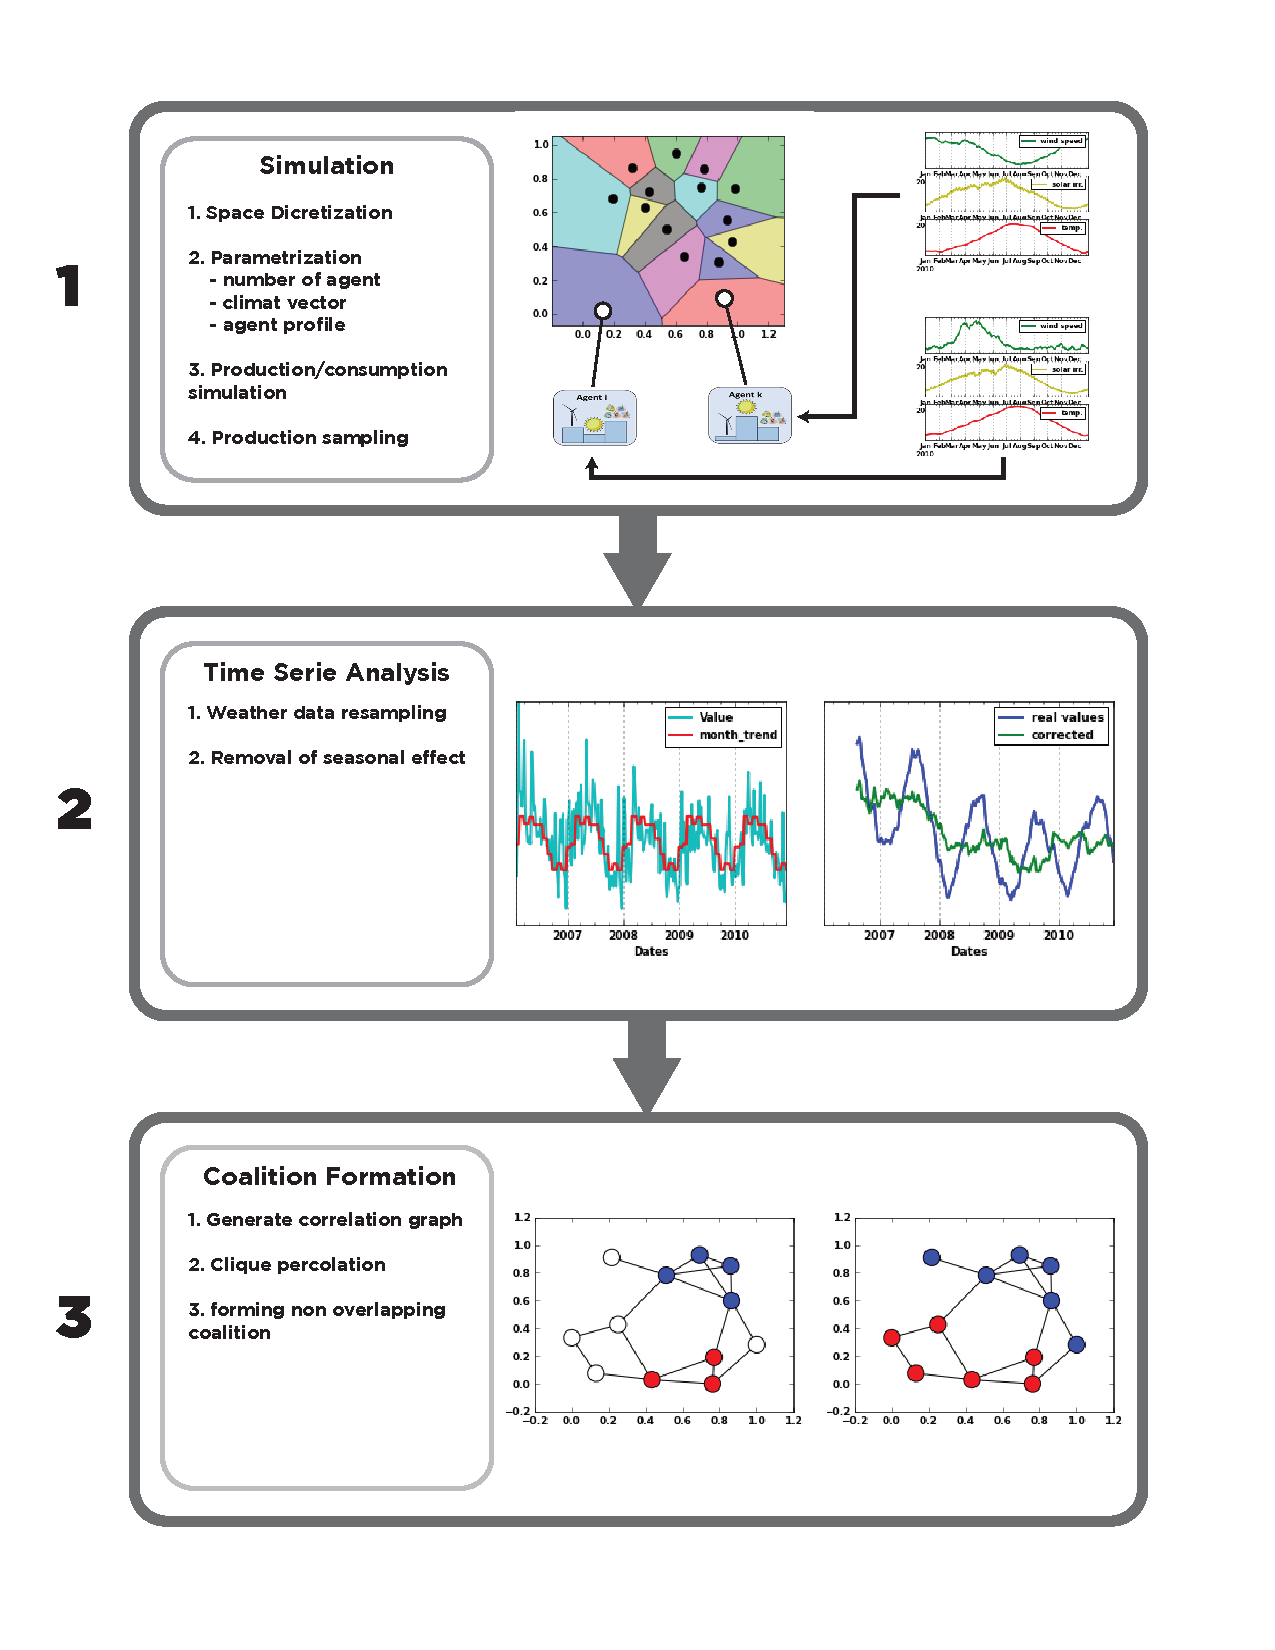
\includegraphics[scale=.39]{Fig2}
		\caption{Process}
		\label{fig:process}
	\end{center}
\end{figure}

An essential component of the smart grid is the smart meter which makes the interface between the end user and the rest of the system. Smart meters coupled with sensors measure quantities of interest (like instantaneous consumption), receive informations from the grid (electricity prices for instance), and take actions accordingly (demand side management programs). Smart meters are currently and gradually deployed, and will probably provide interesting datasets to work on. Unfortunately, at the time this paper was written, production and consumption data for prosumers over a large region were not yet available to our knowledge. Some interesting experiments are nonetheless being conducted and data are progressively made public \cite{ISSDA}. In this paper, we use weather quantities like wind speed or solar radiance as alternative data for generating realistic production and consumption series. Fortunately, these kinds of data are easier to find, and since the development of small personal weather stations, their geographical granularity keeps increasing.  Since these quantities depend both on time and location, we discretize time into slots and space into zones in the following (see block 1 of fig. \ref{fig:process}). A zone is simply a portion of the considered region of study for which we sampled data. Therefore, if prosumers i and j are positioned on the same zone, they are exposed to the same weather. Adding some intra-zone noise can easily be done though not considered in this paper. We denote by $ P_{i}(t) $ the instantaneous available extra-production of agent i at time t :

\begin{figure}
	\begin{center}
		\begin{scriptsize}
		\label{tab:main_notations}
		\begin{tabular}{ | l | r | }
   						N & Number of Prosumers \\
  						$ P_i(t) $ & Extra-production of agent i at time t \\
   						$ P_S^{CRCT} $ & Contract value of coalition S \\
   						$ \phi \in \left[ 0,1 \right] $ & Reliability Threshold \\
   						$ P^{MIN} $ & Minimum Contract value \\
   						$ \alpha $ & Parameter that controls the coalitions sizes \\
   						$ \epsilon $ & Correlation graph filtering threshold \\
   						$ N_{COAL} $ & Number of coalitions \\
   						$ \mathcal{R}_S $ & Resilience of coalition S
 		\end{tabular}
 		\caption{Main notations.}
 	\end{scriptsize}
	\end{center}
\end{figure}

\begin{equation}
P_{i}(t) = P_{i}^{P}(t) - P_{i}^{D}(t)
\end{equation}

Where $ P_{i}^{P}(t) $ represents the total production of agent i at time t and $ P_{i}^{D}(t) $ its consumption at time t. In other words, $ P_{i}(t) $ represents the instantaneous surplus of power that agent i is willing to sell at time t. We simulated these traces by considering separately $ P_{i}^{P} $ and $ P_{i}^{D} $. For a prosumer i, it is possible to write both quantities as a sum over the distributed energy resources ($ DER_{i} $) and loads ($ load_{i} $) of i : 

\begin{equation}
P_{i}^{P}(t) = \sum_{k \in DER_{i}} P_{k}(t)
\end{equation}
\begin{equation}
P_{i}^{D}(t) = \sum_{k \in load_{i}} P_{k}(t)
\end{equation}

For simplicity, in this paper we only consider wind-turbines (WT) and photovoltaic panels (PV) as possible DERs for the agents ($ DER_{i} = WT_{i} \cup PV_{i} $):  

\begin{equation}
P_{i}^{D}(t) = \sum_{k \in WT_{i}} P_{k}(t) + \sum_{k \in PV_{i}} P_{k}(t)
\end{equation} 

We denote by $ \nu_{i}(t) $ and $ \Psi_{i}(t) $ the wind speed (in $ m.s^{-1} $) and the solar radiance ( in $ W.m^{-2} $) at the location of agent i and at time t, so that :
\begin{equation}
 P_{i}^{P}(t) = \sum_{k \in WT_{i}} \mathcal{F}_{WT}( \nu_{i}(t) ) + \sum_{k \in PV_{i} } \mathcal{F}_{PV}(\Psi_{i}(t) ) 
\end{equation}
Where $ \mathcal{F}_{WT} $ (resp. $ \mathcal{F}_{PV} $) is the power curve for the wind-turbines (resp. photovoltaic panels). We made here the implicit assumption that all wind-turbines (resp. photovoltaic panels) have the same power curve. The model can be easily extended to multiple power curves accounting for different types of generators. More details about power curves and their approximations can be found in the appendix and in \cite{Lydia2014}.

Note that a prosumer i is defined by his zone $ Z_{i} $ as well as the sets $ DER_{i} $ and $ load_{i} $. That is, a prosumer can be configured to represent anything from a single wind-turbine for instance ($ DER_{i} = \{ WT_{0} \} $ and $ load_{i} = \emptyset $) to a pure load ($ DER_{i} = \emptyset $ and $ load_{i} = \{ L_{0} \} $) through more complex combinations. In practice, we use random configurations for the agents. In the rest of the paper, we use french weather data \cite{Infoclimat} starting in January 2006 and ending in December 2012, with a sampling frequency of three hours, and generate N timeseries of extra-production over this date range. Note that this low sampling frequency might hide short time intermittencies (see \cite{Anvari2015} for more information). Studying the evolution of the correlation structure with the sampling frequency is out of the scope of this paper, but might lead to interresting results.



%%%%%%%%%%%%%%%%%%%%%%%%%%%%%%%%%%%%%%%%%%%%%%%%%%%%%%%%%%%%%%%%%%%%%%%%%%%%%%%%
%
% Section III: Model
%
%%%%%%%%%%%%%%%%%%%%%%%%%%%%%%%%%%%%%%%%%%%%%%%%%%%%%%%%%%%%%%%%%%%%%%%%%%%%%%%%

\section{Notations}
\label{sec:notations}

This section provides most of the notations and introduces important concepts for the rest of the paper. We consider a set $ \mathcal{A} = \{a_{1},a_{2},...,a_{N} \} $ of N prosumers of the distribution network. Each agent is configured randomly and we simulate its extra-production $ P_{i}(t),\ \forall i \in \mathcal{A} $ from 2006 to 2012. Based on these historical values, our objective is now to form groups of prosumers so that the global power production resulting from the superposition of individual's extra-productions be both sufficiently high and predictable. Let $ P_{S}(t) = \sum_{i \in S} P_{i}(t) $ be the available extra-production of coalition S at time t. 

Suppose now that coalition S has to suggest a production value $ P_{S}^{CRCT} $ to enter the market. This means that, during the time S is on the market, it will have to inject in the grid exactly $ P_{S}^{CRCT} $ at any time t and will be rewarded proportionally to this amount, with penalties if it deviates. Obviously, the actual extra-production will not be constant at this value and will oscillate due to intermittences in the production and consumption. If S has an available production always greater than $ P_{S}^{CRCT} $, it is losing some gains since it could have announced a higher contract value. If the production oscillates around $ P_{S}^{CRCT} $, by using batteries or demand side management techniques, S could be able to maintain its production to the contract value at any time. Nevertheless, if the oscillations are too important compared to the available storage capacity, S will probably break the contract and pay penalties. We can see that there is a return over risk trade-off here. Coalitions should thus find the right balance between announcing too low and losing some potential gains, and claiming too high and paying penalties. 

Let us illustrate the rest of the notations and concepts with a simple example. We consider only two agents i and j such that the distribution of their extra-production can be approximated by normal distributions : $ P_{i} \sim \mathcal{N}(\mu_{i}, \sigma_{i} ) $ and $ P_{j} \sim \mathcal{N}(\mu_{j}, \sigma_{j} ) $. This is only for explanation purposes as it is of course rather unrealistic in real situations where the distributions are skewed. We can write the distribution of the coalition $ S = \{i,j\} $ as $ P_{\{i,j\}} \sim \mathcal{N}(\mu_{ij}, \sigma_{ij}) $, where :

\begin{equation}
\left\{ \begin{array}{lll}
		\mu_{ij} = \mu_{i} + \mu_{j} \\
		\sigma_{ij} = \sqrt{\sigma_{i}^{2} + \sigma_{j}^{2} + \rho_{ij} \sigma_{i} \sigma_{j} }
\end{array} \right.
\end{equation}
$ \rho_{ij} $ being the Pearson's correlation coefficient between $ P_{i} $ and $ P_{j} $. If the coalition $ \{i,j\}$ proposes a contract value $ P_{S}^{CRCT} $, all instants when $ \{i,j\}$ will produce less than $ P_{S}^{CRCT} $ is critical. Indeed, in this kind of situations, $ \{i,j\}$ will either have to discharge batteries to keep up with its contract, or pay penalties to the grid. The probability that $ \{i,j\}$ is under-producing compared to the contract : $ Pr[P_{i,j} \leq P^{CRCT}] $ is thus an important indicator of the coalition's quality. A well-known result for normal distributions is that the cumulative distribution function can be written as :
\begin{equation}
Pr[P_{ij} \leq P_{S}^{CRCT}] = \dfrac{1}{2} \left[ 1+ erf \left( \dfrac{P_{S}^{CRCT} - \mu_{ij}}{\sigma_{ij}\sqrt{2}} \right) \right] 
\end{equation}
where $ erf $ is the error function : $ erf(x) = \dfrac{2}{\sqrt{\pi}}\int_{0}^{x} e^{-t^{2}} dt $.

The contract a given coalition is willing to take depends on its capacity to compensate for under-producing (using batteries, backup generators...), and its risk acceptance. Selecting the right contract value appears thus as an interesting problem on its own that we plan to investigate in future works. In order to keep the present paper in a reasonable length, we simplify the contract value selection problem by giving some responsibilities to a third party named the market operator. His role is to constrain the market entry to coalitions able to propose both sufficiently high and sufficiently credible contract values. More formally, let $ \phi \in [0,1] $ be the reliability threshold fixed by the market operator as a maximum value for the probability of under-producing. The highest contract value that a coalition can propose is thus $ P_{S}^{CRCT \star} $ such that $ Pr[P_{ij} \leq P_{S}^{CRCT \star}] = \phi $. In the Gaussian example, it implies that coalition $ \{i,j\}$ is announcing :

\begin{equation}
\label{eq:P_star}
P_{S}^{CRCT \star} = \mu_{ij} - \sqrt{2} \sigma_{ij} erf^{-1}( 1 - 2 \phi )
\end{equation}

\begin{figure}
	\begin{center}
		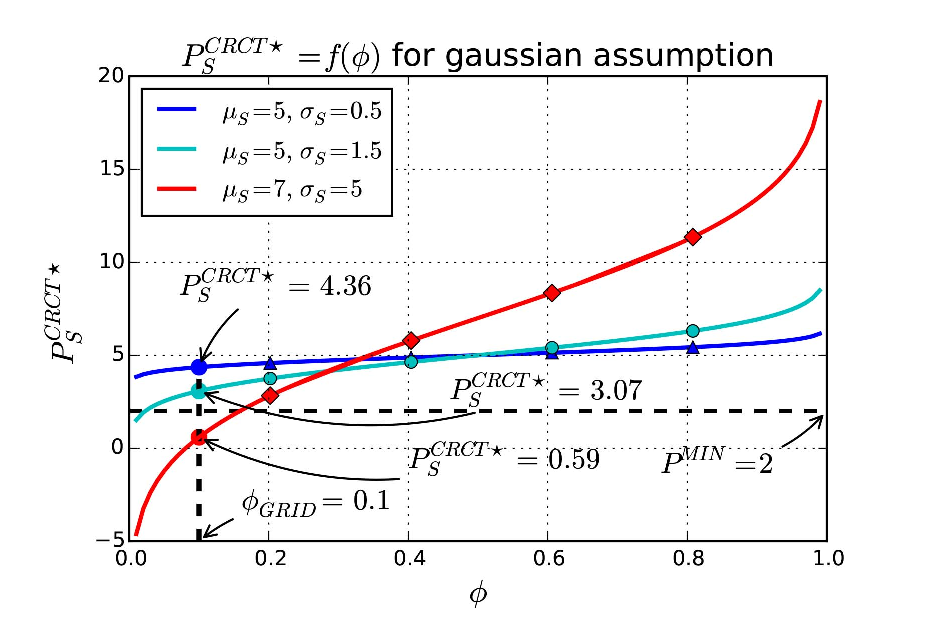
\includegraphics[scale=.46]{./figs/figure_1}
		\caption{{\footnotesize $ P_{S}^{CRCT \star} $ depending on reliability parameter $ \phi $ for Gaussian distributions (see equation \ref{eq:P_star}). Blue curve with triangles stands for a coalition S with an expected production of 5 units and a standard deviation of 0.5. Under a grid policy of $ \phi = 0.1 $, it is able to announce a contract value of $ P_{S}^{CRCT \star} = 4.36 $. The same coalition in term of expected production ($\mu = 5 $), but with a higher variance ($ \sigma = 1.5 $, cyan curve with circles) can only afford a smaller contract value of $ P_{S}^{CRCT \star} = 3.07 $. The red curve with diamonds stands for a coalition with a higher expected production $(\mu = 7)$, but with a very high unpredictability ($ \sigma = 5 $). For low values of $ \phi $, this coalition is thus heavily penalized and can only afford a contract of $ 0.59 $ units. Under grid policy $ (\phi = 0.1, P^{MIN} = 2) $, this last coalition is thus not allowed to enter the market (red dot below the horizontal dashed line).} }
		\label{fig:Gaussian}
	\end{center}
\end{figure}

This is the best contract value that the coalition S can afford for a given stability policy $\phi$ of the market operator. Figure \ref{fig:Gaussian} shows how $ P_{S}^{CRCT \star} $ evolves according to the reliability parameter $ \phi $. For illustration, the range of $ \phi $ values is shown from 0 to 1, but in practice, only small values of $ \phi $ really make sense : $ \phi = 1 $ for instance means that coalitions can announce absolutely anything since the probability of producing less than any contract value is necessarily less than one by trivial definition of a probability. As visible on figure \ref{fig:Gaussian}, coalitions with high expected productions but presenting a high unpredictability are penalized and can only afford small contracts. The market operator also specifies a lower bound $ P^{MIN} $ on the contract values as not to overload the market with unrealistic small coalitions. We thus characterized a valid coalition as one satisfying the two conditions :

\begin{equation}
\left\{ \begin{array}{lll}
			Pr[P_{ij} \leq P_{S}^{CRCT}] \leq \phi \\
			P_{S}^{CRCT} \geq P^{MIN}
\end{array} \right.
\end{equation}

On figure \ref{fig:Gaussian}, $ P^{MIN} $ is fixed to 2 units for illustration purpose. For $ \phi = 0.1 $, only blue triangles and cyan circles coalitions are valid while red diamonds coalition is not.

The Gaussian assumption of this small example is convenient as it allows us to write $ P_{S}^{CRCT \star} $ analytically. Nevertheless, such an assumption is rather unrealistic in practice. In the following, we keep the same framework but release this Gaussian assumption unless the contrary is specified (see eq. \ref{eq:alpha_star}).

%%%%%%%%%%%%%%%%%%%%%%%%%%%%%%%%%%%%%%%%%%%%%%%%%%%%%%%%%%%%%%%%%%%%%%%%%%%%%%%%
%
% Section V: Utility Function
%
%%%%%%%%%%%%%%%%%%%%%%%%%%%%%%%%%%%%%%%%%%%%%%%%%%%%%%%%%%%%%%%%%%%%%%%%%%%%%%%%

\section{Utility Function}
\label{sec:utility}

In this section, we use the notions of contract values and valid coalitions developed in section \ref{sec:notations} in order to design a proper utility function. The contract basically indicates the rate at which a coalition has to inject power in the grid. It seems then natural that coalitions are remunerated proportionally to their contract values $ gain(S) \propto P_{S}^{CRCT \star} $. More precisely, if $ \lambda $ is the unitary price rate for electricity, a coalition S injecting $ P_{S}^{CRCT \star} $ in the grid during a period $ [t_{0},t_{k}] $ earns :

\begin{equation}
gain(S) = \int_{t_{0}}^{t_{k}} \lambda P_{S}^{CRCT \star} dt = P_{S}^{CRCT \star} \int_{t_{0}}^{t_{k}} \lambda dt
\end{equation} 
(since $ P_{S}^{CRCT \star} $ is supposed to be a constant rate over the contracted period). Unfortunately $ gain(S) $ is not a concave function of the coalitions' sizes, meaning that coalitions can grow as large as the number of agents allows it, without any counterbalance effects. Such a model, that virtually allows infinitely large coalitions and contract values, is in practice not realistic. There are indeed costs (communication costs for instance) that increase with the coalitions sizes. We take this observation into account by rescaling the utility of a coalition S by its size in term of number of agents ($|S|$):

\begin{equation}
\mathcal{U}(S) = \left\{ \begin{array}{lll}
							\dfrac{1}{|S|^{\alpha}} \dfrac{ P_{S}^{CRCT \star} }{P^{MAX}},\ if\ S\ is\ valid, \\
							0,\ if\ S\ is\ not\ valid
						 \end{array}
				  \right.
\end{equation}
where parameter $ \alpha $ controls to what extent the size of a coalition impacts its utility, and $ P^{MAX} $ is a normalizing factor. Based on $ \mathcal{U} $, the marginal contribution of an agent i can be expressed as $ \delta_{S}(i) = \mathcal{U}(S+\{i\}) - \mathcal{U}(S) $. A coalition S has thus an interest in adding an additional agent i if : 

\begin{equation}
\delta_{S}(i) \geq 0 \ \ \ \Leftrightarrow \ \ \ P_{S+\{i\}}^{CRCT \star} \geq P_{S}^{CRCT \star} \left( \dfrac{|S|+1}{|S|} \right)^{\alpha}
\label{eq:marginal_benefit}
\end{equation}

If $ \alpha = 0 $, agents are added as long as they increase the contract value of the coalition. If $ \alpha > 0 $, additional agents have to increase the contract value by some factor. 

In real situations, the shape of such utility function might be complex with numerous local maximums. We choose in this paper to favor the exploration of the space around balanced regions, i.e regions where coalitions sizes are relatively balanced. Therefore, we use $ \alpha $ as a proxy for having both a concave utility function and preferences in the search space. Given a situation with N prosumers and $ N_{COAL} $ desired coalitions, we wish to select $ \alpha $ such that the utility function tend to favor coalitions of approximately $ \bar{N}=N/N_{COAL} $ agents.

In the general case where distributions and correlation structures have no special form, finding an analytical expression for $ \alpha $ appears complicated. To overcome this problem, we seek an approximation for $ \alpha $ in a simplified situation where all power distributions are approximated by normal distributions and all prosumers are considered equivalent to a mean agent : $ \forall i \in \mathcal{A},\ P_i \sim \mathcal{N}(\bar{\mu}, \bar{\sigma}) $, where $ \bar{\mu} = \frac{1}{N} \sum_{i \in \mathcal{A}} \mu_i $, $ \bar{ \sigma } = \frac{1}{N} \sum_{i \in \mathcal{A}} \sigma_i $, and $\forall i,j,\ \rho_{ij} = \bar{\rho} $. In this simplified case, we can express the utility as a function of $ \bar{\mu} $, $ \bar{\sigma} $, $\bar{\rho} $, $ \bar{N} $, and $ \alpha $ (see Appendix). We then select $ \alpha^{\star} $ such that :

\begin{equation}
\left\{ \begin{array}{lll}
	          \left[ \dfrac{\partial{ U}}{ \partial{|S|}} \right]_{|S| = \bar{N}} = 0 \\
	          \left[ \dfrac{\partial^2 U}{\partial |S|^2} \right]_{ \alpha = \alpha^{\star} } \leq 0
	    \end{array} 
\right.
\label{eq:derivative}
\end{equation}

Which leads to (see Appendix) :

\footnotesize
\begin{equation}
\alpha^{\star}_{\bar{N}} = \dfrac{0.7 \bar{\sigma}(\bar{\rho}-1)erf^{-1}(2 \phi - 1)}{\bar{\mu}\sqrt{\bar{N}(\bar{\rho}\bar{N}-\bar{\rho}+1)}+1.4 \bar{\sigma} erf^{-1} (2 \phi -1 ) (\bar{\rho}\bar{N}-\bar{\rho} + 1)} 
\label{eq:alpha_star}
\end{equation}
\normalsize

Figure \ref{fig:mean_approx} shows how $ \alpha^{\star} $ and the utility function evolves according to the mean size of the coalitions $ \bar{N} $. Given a policy $ (\phi, P^{MIN} ) $ and a pool of N prosumers, we are now able to quantify the quality of any coalition S.


\begin{figure}
	\begin{center}
		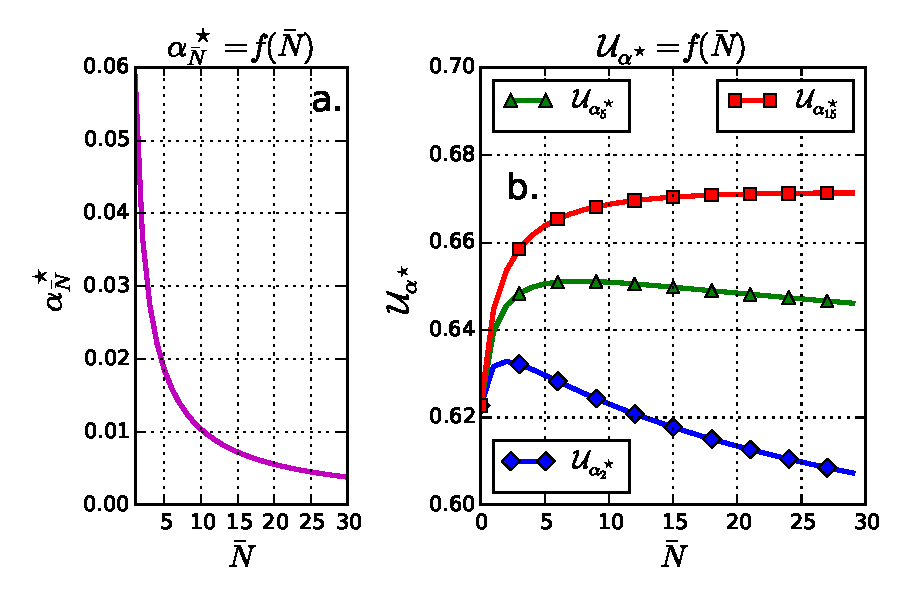
\includegraphics[scale=.46]{./figs/figure_2}
		\caption{{\footnotesize Gaussian mean approximation ($N=100,\ \phi=0.1,\ \bar{\mu}=5,\ \bar{\sigma}=.5,\ \bar{\rho}=0.2 $). Subplot \textbf{a} shows how the parameter $ \alpha $ of the utility function should be chosen in function of the mean size of the coalitions (see equation \ref{eq:alpha_star}). Subplot \textbf{b} displays the corresponding utility functions for different values of $ \alpha $. Blue curve with diamonds favors small coalitions of 2 agents while the green one with triangles favors 5 agents coalitions. Finally, the red curve with squares has an optimal size of 15 agents.} }
		\label{fig:mean_approx}
	\end{center}
\end{figure}

%%%%%%%%%%%%%%%%%%%%%%%%%%%%%%%%%%%%%%%%%%%%%%%%%%%%%%%%%%%%%%%%%%%%%%%%%%%%%%%%
%
% Section VI: Coalition Formation
%
%%%%%%%%%%%%%%%%%%%%%%%%%%%%%%%%%%%%%%%%%%%%%%%%%%%%%%%%%%%%%%%%%%%%%%%%%%%%%%%%
\section{Coalition Formation}
\label{sec:forming}
We aim at forming $ N_{COAL} $ coalitions $ \{ S_1;S_2;...;S_{N_{COAL}} \} $ such that the global utility $ U = \sum_{i = 1}^{N_{COAL}} \mathcal{U}(S_i) $ is maximized. Since achieving such a goal is a well-known hard problem due to the combinatorial explosion in the number of possible aggregations, we propose in this section a greedy heuristic using decorrelation graphs to solve the problem.

\subsection{Representing the correlation structure}
As seen in section \ref{sec:notations}, the variance of the aggregated production impacts directly the contract values, and depends on the covariances between the agents productions. We argue here that, by having some representation of the correlation structure between the agents, the search landscape for high utility coalitions could be reduced, such that good coalitions are more likely to be found quickly. Usually, this correlation structure is formalized with a covariance matrix or a correlation matrix that contains all the correlation coefficients between the agents : $ M = (\rho_{ij})_{\forall i,j \in \mathcal{A}^{2}}$. By using a metric to map this matrix in a weighted adjacency matrix (see section \ref{sec:related}), it is possible to obtain a graph representation of the correlation relationships between the agents. In the following, we use two opposite distance metrics $  d_{ij}^{1} = 1 - \rho_{ij}^{2} $ and $ d_{ij}^{2} = \rho_{ij}^{2} = 1 - d_{ij}^{1} $.


Clearly, $ d^{1} $ (resp. $ d^{2} $) maps two correlated series as close points (resp. distant) while two uncorrelated series are distant (resp. close). These metrics enable us to compute a correlation graph $ G_{1} = (\mathcal{A}, E_{1}) $ and a "de-correlation" graph $ G_{2} = (\mathcal{A}, E_{2} ) $. For any i and j, the weight of the edge $ e_{ij} $ is $ d_{ij}^{1} $ in $ G_{1} $ and $ d_{ij}^{2} $ in $ G_{2} $. In both cases, we want to keep only the edges which weights are located in the lower tail of the distance distributions. In other words, we want to compute the $ \epsilon$-graphs of $ G_{1} $ and $ G_{2} $ such that only meaningful edges remain. Selecting the filter $ \epsilon $ is an important point affecting the landscape search for the coalition formation. Unfortunately, there seems to be no clear consensus in the literature on how to select such a threshold. We will see later in this section that cliques in $ G_{2} $ are potential seeds for the coalitions. Since we want to generate $ N_{COAL} $ coalitions, we need at least $ N_{COAL} $ cliques of a given size to start. Besides, since we consider coalitions as disjoint, the starting cliques should be non overlapping. We select our optimal threshold for $ G_{2} $ as :

\begin{equation}
\label{epsilon_star}
\epsilon^{\star} = min_{ \epsilon \in [0,1]} \left\{ \epsilon\ s.t.\ |\Theta_{k}(G_{2}^{\epsilon})| \geq N_{COAL} \right\}
\end{equation} 
where $ G_{2}^{\epsilon} $ is the de-correlation graph $ G_{2} $ filtered by $ \epsilon $, and $ \Theta_{k}(G) $ is the set of non overlapping cliques of size k in a given graph G. In other words we select $ \epsilon^{\star} $ as the smallest threshold possible such that the filtered de-correlation graph contains at least $ N_{COAL} $ non overlapping cliques of size k. In practice, since finding cliques requires exponential time, we use triangles \cite{Schank2001} ($k=3$ in eq. \ref{epsilon_star}) rather than cliques as soon as the number of nodes is not small. Note also that the existence of $ \epsilon^{\star} $  as defined in equation  \ref{epsilon_star} is not guaranteed.

\subsection{Cliques}

In \cite{Garas2008} the structural roles of weak and strong links on financial correlation graphs is investigated. The author shows that strong links, accounting for strong correlation relationships, are responsible for the clustering, while weak links provide the connectivity between clusters. Indeed, if we consider three items, say a, b, and c such that a and b are strongly correlated and b and c are also strongly correlated, then it is likely that a and c are also strongly correlated. It can be easily shown using the cosine addition formula\footnote{ $ cos(a+b) = cos(a)cos(b) - sin(a)sin(b) $ }, that if $\rho_{ab} > x $ and $\rho_{bc} > x $ with $ x>0 $, then $\rho_{ac} > 2x^{2}-1$). Correlation graphs capture this weak transitivity notion through clusters of correlated series.

Nevertheless de-correlation seems like a more complex concept than correlation in the sense that there is not even a partial notion of transitivity when it comes to it. Therefore, the clustering coefficients of $ G_{1}^{\epsilon} $ is much higher than the one of $ G_{2}^{\epsilon} $. This can be seen as another formulation of \cite{Garas2008} on the structural roles of weak and strong links on financial correlation graphs. Strong links, accounting for strong correlation relationships, are responsible for the clustering, while weak links provide the connectivity between clusters. Searching for clusters in $ G_{2}^{\epsilon} $ and hoping that this strategy will provide a nice coalition structure of internally uncorrelated coalitions seems thus pointless. Consider now a clique in  $ G_{2}^{\epsilon} $, which is a complete subgraph of $ G_{2}^{\epsilon} $. Since there is a link for every pairs of nodes, we know, by construction, that a clique has a mean correlation and a maximum correlation less than $ \epsilon $. 

\begin{figure}
	\begin{center}
		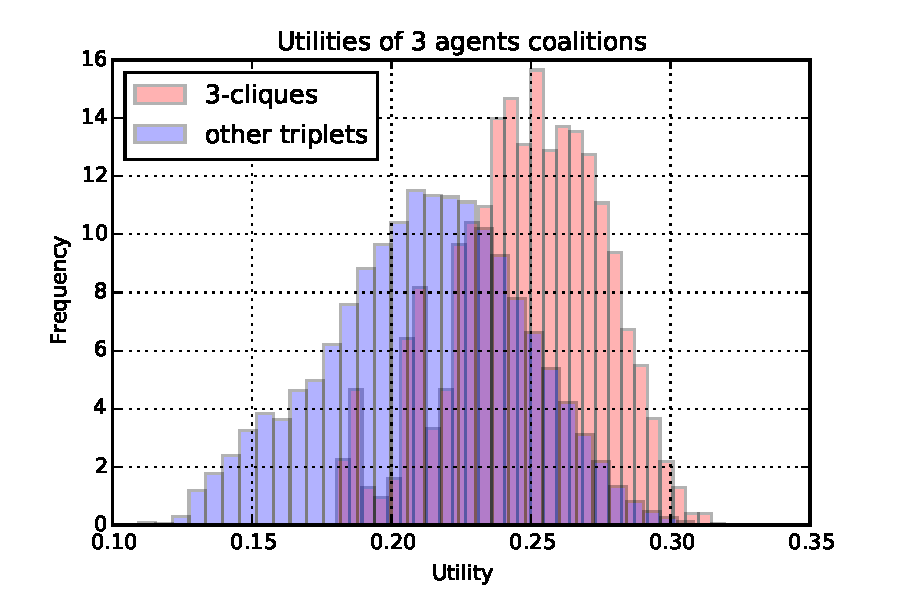
\includegraphics[scale=.45]{./figs/figure_3}
		\caption{{\footnotesize Histograms of utility values for coalitions of size 3 ($\bar{N}=3$) in a $N=200$ prosumers example ($\phi = 0.1$, $ \alpha^{\star} = 0.08 $, $ \bar{\mu}=3.9\ MW $, $\bar{\sigma} = 1.9 MW $, $ \bar{\rho} = 0.69 $). Red bars stand for cliques in the decorrelation graph, and blue bars for all the other possible triples. Cliques tend to exhibit higher utilities than random coalitions.}}
		\label{fig:histo_cliques}
	\end{center}
\end{figure}

Figure \ref{fig:histo_cliques} shows the distributions of the utility values for cliques of size 3 (triangles) in $ G_{2}^{\epsilon^{\star}} $ and for all the other possible triplets of agents. It is clearly visible that cliques tend to exhibit higher utilities because of their de-correlation property. Choosing cliques in $ G_{2}^{\epsilon^{\star}} $ as coalitions seems therefore appealing. Nevertheless, the quality of the results seems to decrease as the sizes of the cliques increase. Indeed, the larger the desired cliques, the more dense $ G_{2}^{\epsilon^{\star}} $ becomes (see equation \ref{epsilon_star}). There is a point where cliques result more from noisy edges than true de-correlation, which decreases the quality of the results. Directly mapping cliques to coalitions by this de-correlation oriented approach is thus not sufficient. It is indeed possible that adding agents to these cliques has the combined effect of increasing the expected production while decreasing its stability. The question revolves around measuring the benefits of this production surplus compared to the disadvantage of having coalition with high volatility. This can be quantified by the marginal benefit in equation \ref{eq:marginal_benefit}.

\subsection{Algorithm}
The algorithm takes inputs from :

\begin{itemize}
	\item \textbf{The agents :} historical series of available productions $P_{i}$, 
	\item \textbf{The market operator :} market entrance policy $ (P^{MIN},\phi) $,
	\item \textbf{The "user" :} Number of desired coalitions $ N_{COAL} $ and size of starting cliques k.
\end{itemize} 

The first steps consist in computing the de-correlation graph $ G_{2} $ as well as the optimal threshold $ \epsilon^{\star} $. Cliques of size k in $ G_{2}^{\epsilon^{\star}} $ are considered as coalition seeds. The next step is a local greedy improvement over the landscape represented by  $ G_{2}^{\epsilon^{\star}} $. Cliques add alternatively the node $ i^{\star} $ in their neighborhood that yields the best marginal benefit $ MAX_{ i \in N(clique) } \delta_{clique}(i) $ where $ N(clique) $ is the neighborhood of a given clique. See algorithms section in the appendix.


%%%%%%%%%%%%%%%%%%%%%%%%%%%%%%%%%%%%%%%%%%%%%%%%%%%%%%%%%%%%%%%%%%%%%%%%%%%%%%%%
%
% Section VII: Results
%
%%%%%%%%%%%%%%%%%%%%%%%%%%%%%%%%%%%%%%%%%%%%%%%%%%%%%%%%%%%%%%%%%%%%%%%%%%%%%%%%
\section{Results}
\label{sec:results}

The algorithm presented in the previous section is supposed to generate a given number of coalitions that have good utilities. As it comprises mainly of a greedy optimization based on local improvements, there is no guarantee that the algorithm finds the global optimum. Since there is, to our knowledge, no state of the art algorithm that aggregates uncorrelated agents in an optimum way (see section \ref{sec:related} for related problems), we compare the results with :

\begin{itemize}
\item \textbf{Random sampling of coalitions :} Coalitions are formed randomly without any other constraint that the desired size. This enables us to have an idea about the distributions of utility values for coalitions of a given size.
\item \textbf{Random sampling of coalition structures :} Coalition structures are sampled randomly by shuffling and random divisions of the agents. This algorithm (see appendices) uses such a sampling and returns the highest utility coalition structure sampled. We refer to this algorithm as "\textit{random}".
\item \textbf{Correlated :} Opposite version of our algorithm. It performs a community detection on the correlation graph $ G_{1} $. The resulting coalitions have thus very high internal correlations. We thus expect this algorithm to perform very bad compared to the others. See appendices.
\end{itemize} 


Before running the algorithms, we need to calibrate the utility function by choosing the value of the $ \alpha $ parameter. Recall that the purpose of this parameter is to take into account some constraints on the coalition's sizes if needed. In this paper, we do not have any technical constraints on coalition sizes though we designed the utility such that these could be taken into account. We select the desired size as being $ \lfloor N/N_{COAL} \rfloor $ (where $ \lfloor.\rfloor $ means floor). Figure \ref{fig:real_utility2} shows how the mean utility of a coalition evolves with its size when the optimum size is set to 40 agents.


\begin{figure}
	\begin{center}
		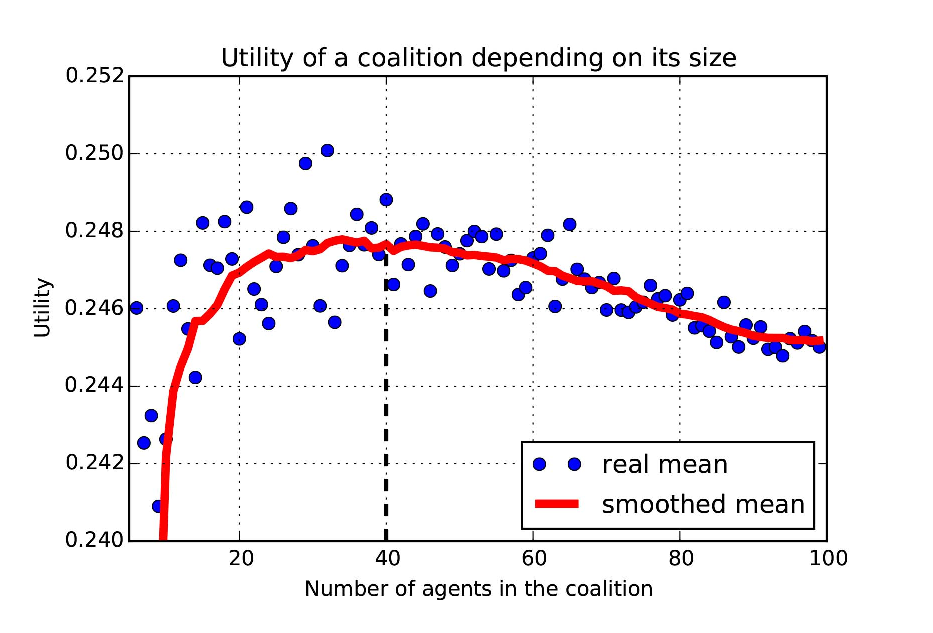
\includegraphics[scale=.45]{./figs/figure_4}
		\caption{{\footnotesize Utility of random coalitions depending on their size in a $N=200$ prosumers example ($\phi = .1$, $ \bar{\mu}=3.9\ MW $, $\bar{\sigma} = 1.9 MW $, $ \bar{\rho} = 0.69 $). Blue dots show real mean utility values and the thick red curve its smoothed version by applying a Savitzky-Golay filter. On this plot, $ \alpha^{\star} = 0.006 $, and was selected according to eq. \ref{eq:alpha_star} in order to favor $\bar{N} = 40$ agents coalitions.}}
		\label{fig:real_utility2}
	\end{center}
\end{figure}


Figure \ref{fig:coalitions} shows the coalitions formed with the considered algorithms in the contract value / volatility space. The color map in the background indicates regions where we expect high utilities (red) and the ones where we expect very poor utility values (blue). The bottom right corner, with high contract values and low volatilities, is therefore the region where we wish to form our coalitions. A single coalition is represented by a marker and the color and shape of a marker indicates by which algorithm the coalition has been formed. Besides, the sizes of the coalitions are indicated on the markers, and the marker size is also proportional to the coalition size. We can see that the utility function results in approximatively balanced coalitions. Small yellow markers indicates the gravity centers of their respective coalition structures. The coalitions of correlated agents (green squares) are clearly of poor quality according to our criteria since they can only afford small production contracts, and with a very high volatility. The decorrelated coalitions (blue dots) are closer to the bottom right corner indicating a much better quality in term of productivity over volatility ratio. The black dotted line indicates the mean values for the random coalitions sampling technique. Each small dot stands for the mean position of all sampled coalitions of this given size. Variances are not indicated for readability, but are usually quite large since this sampling only takes the size as a constraint. We can see that as coalitions get larger, they tend to increase on average their contract values, but at the price of a higher volatility. The results of the random coalition structure sampling are shown with the red ellipses that represent the distribution of the gravity centers of the sampled structures. Since the center of the ellipses stands for the mean and each ellipse adds one standard deviation, more than $ 99\% $ of the sampled gravity centers are within the largest ellipse. The small yellow dot below the ellipses indicates the gravity center of our solution. It is thus visible that our greedy graph based algorithm is able to find a quite good coalition structure in terms of volatility and contract values.

\begin{figure}
	\begin{center}
		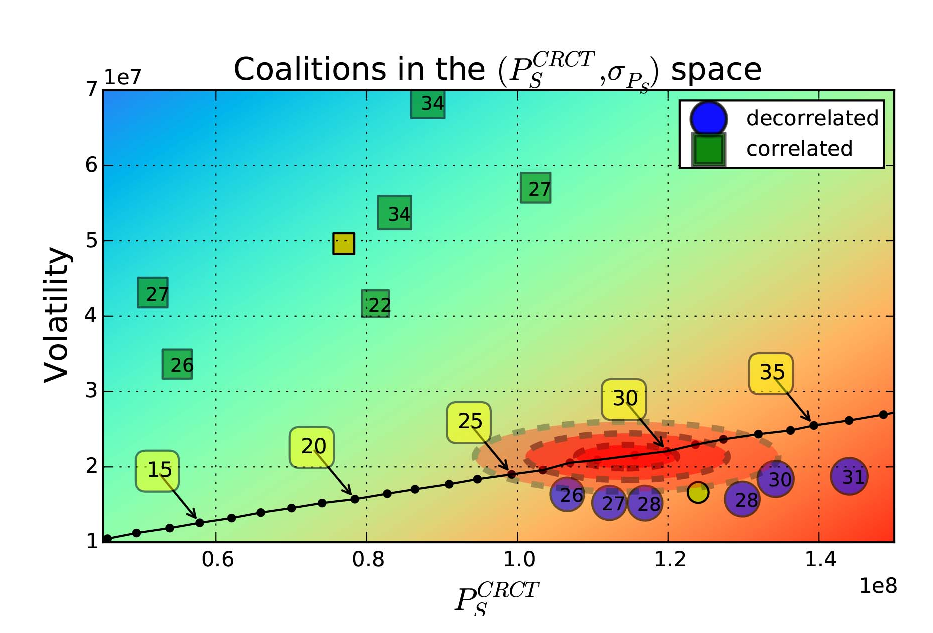
\includegraphics[scale=.45]{./figs/figure_5}
		\caption{{\footnotesize Coalitions formed in the (contract value, volatility) space. The color map indicates the underlying quality. The closer to red the better (high contract values with small volatility). On the opposite, blue areas show poor quality (small contract values with high volatility). Blue dots stand for the decorrelated coalitions that we formed while green squares show correlated coalitions. The smaller yellow markers stand for the gravity centers of the coalition structures. The black dotted line shows how contract values and volatility evolve  when the size of the coalitions increases (a subset of the points are labeled by the size of the coalition they represent). Each point is the average over $ 10^{5} $ unconstrained draws of a random coalition. We also show the distribution of the gravity centers of random coalition structures with red ellipses (center is the mean, and each ellipse corresponds to one  standard deviation).}}
		\label{fig:coalitions}
	\end{center}
\end{figure}

A key point for the coalitions, besides stability and productivity, is their resilience. The resilience of a system refers to its ability to perform its tasks when subject to failures of its components. We consider here the case of random failures of the power electronics of some agents that has the consequence of preventing them from participating in the market. Therefore, the notion of resilience we will use in the following can be seen as the ability of the coalition structures to inject stable power in the grid when some of its internal agents are removed. According to our model, the market operator specified two thresholds ($P^{MIN}$ and $ \phi $) such that the power injected by every coalition is constrained : $ P_{S}^{CRCT} \in [P^{MIN}, P_{S}^{CRCT \star}] $. As long as a coalition can propose a contract value higher than $ P^{MIN} $, it is valid and allowed to enter the energy market. We define the resilience of a coalition S as the probability that S produces more than the $ P^{MIN} $ threshold : $ \mathcal{R}_{S} = Pr[P_{S} >= P^{MIN}] = 1 - Pr[P_{S} < P^{MIN}] $. And we extend this measure to the coalition structures :

\begin{equation}
\mathcal{R}_{CS} = \prod_{S \in CS} \left( 1 - Pr[ P_{S} < P^{MIN} ] \right)
\label{eq:resilience}
\end{equation}

We consider that prosumers fail randomly, and we denote by $ \psi \in [0,1] $ the fraction of agents that failed. Figure \ref{fig:resilience} exhibits how the resilience of the coalition structures evolves according to $ \psi $ (see appendix section \textit{Resilience algorithm} for more details). On the top subplot, $ P^{MIN} $ was voluntarily selected relatively low such that the resiliences of the three structures fit on the same figure. When the $ P^{MIN} $ requirement increases, the differences between the algorithms also increase as visible on the bottom subplot of figure \ref{fig:resilience}. The decorrelated coalitions achieve a more resilient production on the market in the sense that they sustain a higher fraction of node failures.

\begin{figure}
	\begin{center}
		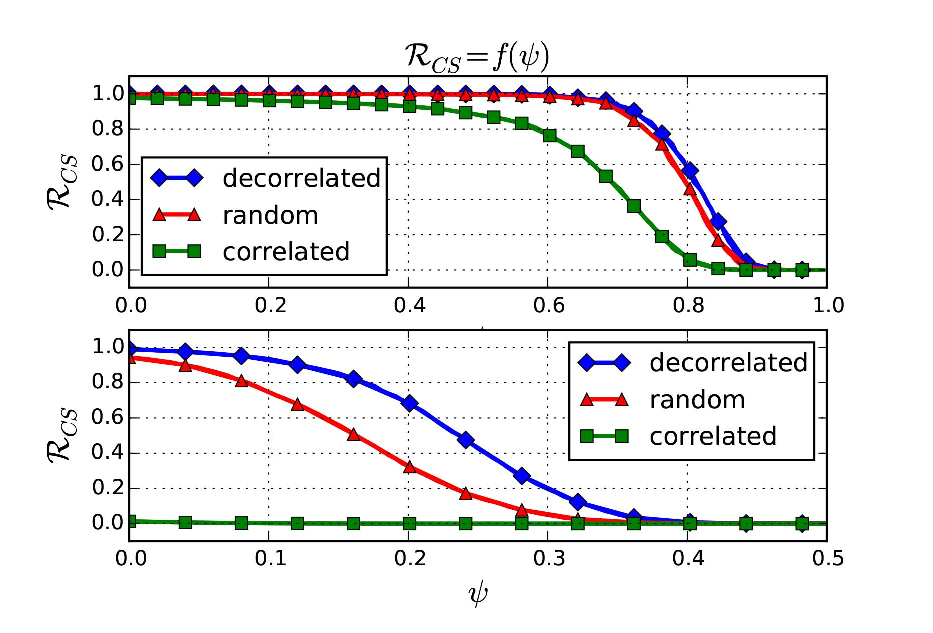
\includegraphics[scale=.45]{./figs/figure_6}
		\caption{{\footnotesize Resilience of the coalition structures when nodes fail randomly (see equation \ref{eq:resilience}) for $ P^{MIN} = 10MW $ (top subplot) and $ P^{MIN} = 80MW $ (bottom subplot)} }
		\label{fig:resilience}
	\end{center}
\end{figure}

%%%%%%%%%%%%%%%%%%%%%%%%%%%%%%%%%%%%%%%%%%%%%%%%%%%%%%%%%%%%%%%%%%%%%%%%%%%%%%%%
%
% Section VI: Conclusion
%
%%%%%%%%%%%%%%%%%%%%%%%%%%%%%%%%%%%%%%%%%%%%%%%%%%%%%%%%%%%%%%%%%%%%%%%%%%%%%%%%
\section{Conclusion}
\label{sec:conclusion}

In this paper we studied how aggregations of prosumers could be authorized to sell their surplus of production on the energy market. By relying on the past values of the agents, we constrained the market entry to both sufficiently productive and stable coalitions. The power that a coalition is able to propose on the market is therefore related to production and stability. The correlations between the prosumers impact directly the volatility of the coalitions, which led us to seek uncorrelated aggregations of agents. We used a graph representation of the correlation relationships between the agents as a reduced landscape for the coalition formation. A greedy algorithm that starts with cliques of the "de-correlation" graph of the agents and makes local improvements offers a good compromise between speed and quality of the results. We compared these results with random samplings, and an opposite strategy that clusters correlated agents together. We showed that the coalitions resulting from our algorithm are able to provide more power to the grid with a lower volatility. Because of their better production over volatility ratios, these coalitions will tend to use less storage and waste less energy than more unstable coalitions. Because in real situations, agents are prone to failure, resilience is also an important criterion for the quality of the aggregations. We therefore studied how the coalitions remain on the market when their agents fail randomly. We showed that, in this situation, the coalitions resulting from our algorithm better withstand losses of agents. A possible direction for future work could be to use, in addition to real weather data, data from energy markets and aggregators as to propose a prosumer aggregation model closer to real conditions.

%%%%%%%%%%%%%%%%%%%%%%%%%%%%%%%%%%%%%%%%%%%%%%%%%%%%%%%%%%%%%%%%%%%%%%%%%%%%%%%%
%
% Bibliography
%
%%%%%%%%%%%%%%%%%%%%%%%%%%%%%%%%%%%%%%%%%%%%%%%%%%%%%%%%%%%%%%%%%%%%%%%%%%%%%%%%

\bibliographystyle{IEEEtran}  
\bibliography{Article}



\end{document}


